% Generated by Sphinx.
\def\sphinxdocclass{report}
\documentclass[letterpaper,10pt,english]{sphinxmanual}
\usepackage[utf8]{inputenc}
\DeclareUnicodeCharacter{00A0}{\nobreakspace}
\usepackage{cmap}
\usepackage[T1]{fontenc}
\usepackage{babel}
\usepackage{times}
\usepackage[Bjarne]{fncychap}
\usepackage{longtable}
\usepackage{sphinx}
\usepackage{multirow}


\title{reST Documentation}
\date{January 26, 2015}
\release{1}
\author{Lamfung Wen}
\newcommand{\sphinxlogo}{}
\renewcommand{\releasename}{Release}
\makeindex

\makeatletter
\def\PYG@reset{\let\PYG@it=\relax \let\PYG@bf=\relax%
    \let\PYG@ul=\relax \let\PYG@tc=\relax%
    \let\PYG@bc=\relax \let\PYG@ff=\relax}
\def\PYG@tok#1{\csname PYG@tok@#1\endcsname}
\def\PYG@toks#1+{\ifx\relax#1\empty\else%
    \PYG@tok{#1}\expandafter\PYG@toks\fi}
\def\PYG@do#1{\PYG@bc{\PYG@tc{\PYG@ul{%
    \PYG@it{\PYG@bf{\PYG@ff{#1}}}}}}}
\def\PYG#1#2{\PYG@reset\PYG@toks#1+\relax+\PYG@do{#2}}

\expandafter\def\csname PYG@tok@gd\endcsname{\def\PYG@tc##1{\textcolor[rgb]{0.63,0.00,0.00}{##1}}}
\expandafter\def\csname PYG@tok@gu\endcsname{\let\PYG@bf=\textbf\def\PYG@tc##1{\textcolor[rgb]{0.50,0.00,0.50}{##1}}}
\expandafter\def\csname PYG@tok@gt\endcsname{\def\PYG@tc##1{\textcolor[rgb]{0.00,0.27,0.87}{##1}}}
\expandafter\def\csname PYG@tok@gs\endcsname{\let\PYG@bf=\textbf}
\expandafter\def\csname PYG@tok@gr\endcsname{\def\PYG@tc##1{\textcolor[rgb]{1.00,0.00,0.00}{##1}}}
\expandafter\def\csname PYG@tok@cm\endcsname{\let\PYG@it=\textit\def\PYG@tc##1{\textcolor[rgb]{0.25,0.50,0.56}{##1}}}
\expandafter\def\csname PYG@tok@vg\endcsname{\def\PYG@tc##1{\textcolor[rgb]{0.73,0.38,0.84}{##1}}}
\expandafter\def\csname PYG@tok@m\endcsname{\def\PYG@tc##1{\textcolor[rgb]{0.13,0.50,0.31}{##1}}}
\expandafter\def\csname PYG@tok@mh\endcsname{\def\PYG@tc##1{\textcolor[rgb]{0.13,0.50,0.31}{##1}}}
\expandafter\def\csname PYG@tok@cs\endcsname{\def\PYG@tc##1{\textcolor[rgb]{0.25,0.50,0.56}{##1}}\def\PYG@bc##1{\setlength{\fboxsep}{0pt}\colorbox[rgb]{1.00,0.94,0.94}{\strut ##1}}}
\expandafter\def\csname PYG@tok@ge\endcsname{\let\PYG@it=\textit}
\expandafter\def\csname PYG@tok@vc\endcsname{\def\PYG@tc##1{\textcolor[rgb]{0.73,0.38,0.84}{##1}}}
\expandafter\def\csname PYG@tok@il\endcsname{\def\PYG@tc##1{\textcolor[rgb]{0.13,0.50,0.31}{##1}}}
\expandafter\def\csname PYG@tok@go\endcsname{\def\PYG@tc##1{\textcolor[rgb]{0.20,0.20,0.20}{##1}}}
\expandafter\def\csname PYG@tok@cp\endcsname{\def\PYG@tc##1{\textcolor[rgb]{0.00,0.44,0.13}{##1}}}
\expandafter\def\csname PYG@tok@gi\endcsname{\def\PYG@tc##1{\textcolor[rgb]{0.00,0.63,0.00}{##1}}}
\expandafter\def\csname PYG@tok@gh\endcsname{\let\PYG@bf=\textbf\def\PYG@tc##1{\textcolor[rgb]{0.00,0.00,0.50}{##1}}}
\expandafter\def\csname PYG@tok@ni\endcsname{\let\PYG@bf=\textbf\def\PYG@tc##1{\textcolor[rgb]{0.84,0.33,0.22}{##1}}}
\expandafter\def\csname PYG@tok@nl\endcsname{\let\PYG@bf=\textbf\def\PYG@tc##1{\textcolor[rgb]{0.00,0.13,0.44}{##1}}}
\expandafter\def\csname PYG@tok@nn\endcsname{\let\PYG@bf=\textbf\def\PYG@tc##1{\textcolor[rgb]{0.05,0.52,0.71}{##1}}}
\expandafter\def\csname PYG@tok@no\endcsname{\def\PYG@tc##1{\textcolor[rgb]{0.38,0.68,0.84}{##1}}}
\expandafter\def\csname PYG@tok@na\endcsname{\def\PYG@tc##1{\textcolor[rgb]{0.25,0.44,0.63}{##1}}}
\expandafter\def\csname PYG@tok@nb\endcsname{\def\PYG@tc##1{\textcolor[rgb]{0.00,0.44,0.13}{##1}}}
\expandafter\def\csname PYG@tok@nc\endcsname{\let\PYG@bf=\textbf\def\PYG@tc##1{\textcolor[rgb]{0.05,0.52,0.71}{##1}}}
\expandafter\def\csname PYG@tok@nd\endcsname{\let\PYG@bf=\textbf\def\PYG@tc##1{\textcolor[rgb]{0.33,0.33,0.33}{##1}}}
\expandafter\def\csname PYG@tok@ne\endcsname{\def\PYG@tc##1{\textcolor[rgb]{0.00,0.44,0.13}{##1}}}
\expandafter\def\csname PYG@tok@nf\endcsname{\def\PYG@tc##1{\textcolor[rgb]{0.02,0.16,0.49}{##1}}}
\expandafter\def\csname PYG@tok@si\endcsname{\let\PYG@it=\textit\def\PYG@tc##1{\textcolor[rgb]{0.44,0.63,0.82}{##1}}}
\expandafter\def\csname PYG@tok@s2\endcsname{\def\PYG@tc##1{\textcolor[rgb]{0.25,0.44,0.63}{##1}}}
\expandafter\def\csname PYG@tok@vi\endcsname{\def\PYG@tc##1{\textcolor[rgb]{0.73,0.38,0.84}{##1}}}
\expandafter\def\csname PYG@tok@nt\endcsname{\let\PYG@bf=\textbf\def\PYG@tc##1{\textcolor[rgb]{0.02,0.16,0.45}{##1}}}
\expandafter\def\csname PYG@tok@nv\endcsname{\def\PYG@tc##1{\textcolor[rgb]{0.73,0.38,0.84}{##1}}}
\expandafter\def\csname PYG@tok@s1\endcsname{\def\PYG@tc##1{\textcolor[rgb]{0.25,0.44,0.63}{##1}}}
\expandafter\def\csname PYG@tok@gp\endcsname{\let\PYG@bf=\textbf\def\PYG@tc##1{\textcolor[rgb]{0.78,0.36,0.04}{##1}}}
\expandafter\def\csname PYG@tok@sh\endcsname{\def\PYG@tc##1{\textcolor[rgb]{0.25,0.44,0.63}{##1}}}
\expandafter\def\csname PYG@tok@ow\endcsname{\let\PYG@bf=\textbf\def\PYG@tc##1{\textcolor[rgb]{0.00,0.44,0.13}{##1}}}
\expandafter\def\csname PYG@tok@sx\endcsname{\def\PYG@tc##1{\textcolor[rgb]{0.78,0.36,0.04}{##1}}}
\expandafter\def\csname PYG@tok@bp\endcsname{\def\PYG@tc##1{\textcolor[rgb]{0.00,0.44,0.13}{##1}}}
\expandafter\def\csname PYG@tok@c1\endcsname{\let\PYG@it=\textit\def\PYG@tc##1{\textcolor[rgb]{0.25,0.50,0.56}{##1}}}
\expandafter\def\csname PYG@tok@kc\endcsname{\let\PYG@bf=\textbf\def\PYG@tc##1{\textcolor[rgb]{0.00,0.44,0.13}{##1}}}
\expandafter\def\csname PYG@tok@c\endcsname{\let\PYG@it=\textit\def\PYG@tc##1{\textcolor[rgb]{0.25,0.50,0.56}{##1}}}
\expandafter\def\csname PYG@tok@mf\endcsname{\def\PYG@tc##1{\textcolor[rgb]{0.13,0.50,0.31}{##1}}}
\expandafter\def\csname PYG@tok@err\endcsname{\def\PYG@bc##1{\setlength{\fboxsep}{0pt}\fcolorbox[rgb]{1.00,0.00,0.00}{1,1,1}{\strut ##1}}}
\expandafter\def\csname PYG@tok@mb\endcsname{\def\PYG@tc##1{\textcolor[rgb]{0.13,0.50,0.31}{##1}}}
\expandafter\def\csname PYG@tok@ss\endcsname{\def\PYG@tc##1{\textcolor[rgb]{0.32,0.47,0.09}{##1}}}
\expandafter\def\csname PYG@tok@sr\endcsname{\def\PYG@tc##1{\textcolor[rgb]{0.14,0.33,0.53}{##1}}}
\expandafter\def\csname PYG@tok@mo\endcsname{\def\PYG@tc##1{\textcolor[rgb]{0.13,0.50,0.31}{##1}}}
\expandafter\def\csname PYG@tok@kd\endcsname{\let\PYG@bf=\textbf\def\PYG@tc##1{\textcolor[rgb]{0.00,0.44,0.13}{##1}}}
\expandafter\def\csname PYG@tok@mi\endcsname{\def\PYG@tc##1{\textcolor[rgb]{0.13,0.50,0.31}{##1}}}
\expandafter\def\csname PYG@tok@kn\endcsname{\let\PYG@bf=\textbf\def\PYG@tc##1{\textcolor[rgb]{0.00,0.44,0.13}{##1}}}
\expandafter\def\csname PYG@tok@o\endcsname{\def\PYG@tc##1{\textcolor[rgb]{0.40,0.40,0.40}{##1}}}
\expandafter\def\csname PYG@tok@kr\endcsname{\let\PYG@bf=\textbf\def\PYG@tc##1{\textcolor[rgb]{0.00,0.44,0.13}{##1}}}
\expandafter\def\csname PYG@tok@s\endcsname{\def\PYG@tc##1{\textcolor[rgb]{0.25,0.44,0.63}{##1}}}
\expandafter\def\csname PYG@tok@kp\endcsname{\def\PYG@tc##1{\textcolor[rgb]{0.00,0.44,0.13}{##1}}}
\expandafter\def\csname PYG@tok@w\endcsname{\def\PYG@tc##1{\textcolor[rgb]{0.73,0.73,0.73}{##1}}}
\expandafter\def\csname PYG@tok@kt\endcsname{\def\PYG@tc##1{\textcolor[rgb]{0.56,0.13,0.00}{##1}}}
\expandafter\def\csname PYG@tok@sc\endcsname{\def\PYG@tc##1{\textcolor[rgb]{0.25,0.44,0.63}{##1}}}
\expandafter\def\csname PYG@tok@sb\endcsname{\def\PYG@tc##1{\textcolor[rgb]{0.25,0.44,0.63}{##1}}}
\expandafter\def\csname PYG@tok@k\endcsname{\let\PYG@bf=\textbf\def\PYG@tc##1{\textcolor[rgb]{0.00,0.44,0.13}{##1}}}
\expandafter\def\csname PYG@tok@se\endcsname{\let\PYG@bf=\textbf\def\PYG@tc##1{\textcolor[rgb]{0.25,0.44,0.63}{##1}}}
\expandafter\def\csname PYG@tok@sd\endcsname{\let\PYG@it=\textit\def\PYG@tc##1{\textcolor[rgb]{0.25,0.44,0.63}{##1}}}

\def\PYGZbs{\char`\\}
\def\PYGZus{\char`\_}
\def\PYGZob{\char`\{}
\def\PYGZcb{\char`\}}
\def\PYGZca{\char`\^}
\def\PYGZam{\char`\&}
\def\PYGZlt{\char`\<}
\def\PYGZgt{\char`\>}
\def\PYGZsh{\char`\#}
\def\PYGZpc{\char`\%}
\def\PYGZdl{\char`\$}
\def\PYGZhy{\char`\-}
\def\PYGZsq{\char`\'}
\def\PYGZdq{\char`\"}
\def\PYGZti{\char`\~}
% for compatibility with earlier versions
\def\PYGZat{@}
\def\PYGZlb{[}
\def\PYGZrb{]}
\makeatother

\renewcommand\PYGZsq{\textquotesingle}

\begin{document}

\maketitle
\tableofcontents
\phantomsection\label{index::doc}


Contents:


\chapter{Conference Call Flow}
\label{conf_callflow:conference-call-flow}\label{conf_callflow::doc}\label{conf_callflow:welcome-to-lamfung-s-documentation}
This document will show you the following concept:
\begin{itemize}
\item {} 
Start a meeting

\item {} 
Join a meeting

\item {} 
Leave a meeting

\item {} 
End a meeting

\item {} 
Lock a meeting

\end{itemize}


\section{GetPingServerList}
\label{conf_callflow:getpingserverlist}\begin{itemize}
\item {} 
GetPrimaryPingServerList

\item {} 
GetBackupPingServerList

\end{itemize}


\chapter{Application Share Up Layer Logic}
\label{app_share:application-share-up-layer-logic}\label{app_share::doc}
In this document you will learn:
\begin{itemize}
\item {} 
How to show the running dialog

\item {} 
How to show the installed dialog

\item {} 
How the presenter start share application

\item {} 
How the attendee will do when he received application shared notify message

\end{itemize}


\section{Show Running Dialog}
\label{app_share:show-running-dialog}
Here is the TC sequence

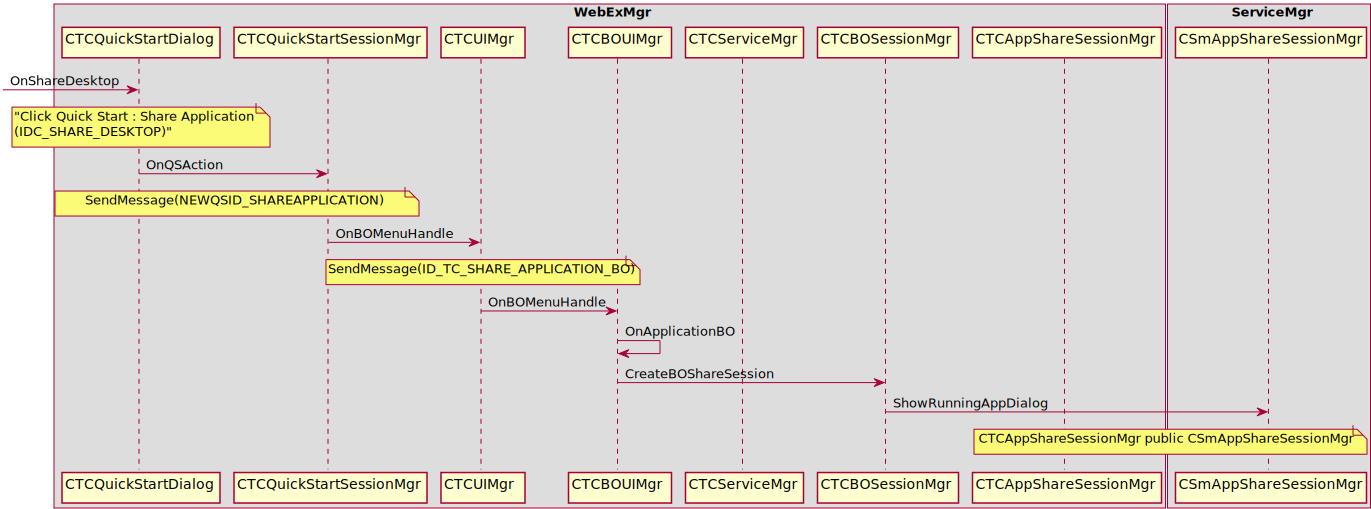
\includegraphics{quick_start_share_application_seq.svg}


\section{Show Installed Dialog}
\label{app_share:show-installed-dialog}
Show More Menu:

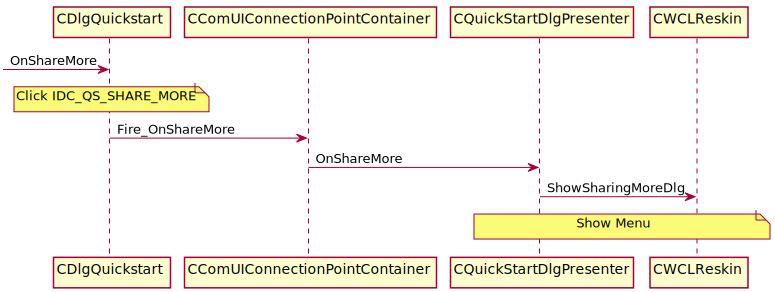
\includegraphics{quick_start_share_application_more_menu_seq.svg}

Show \textbf{Other Application} Dialog

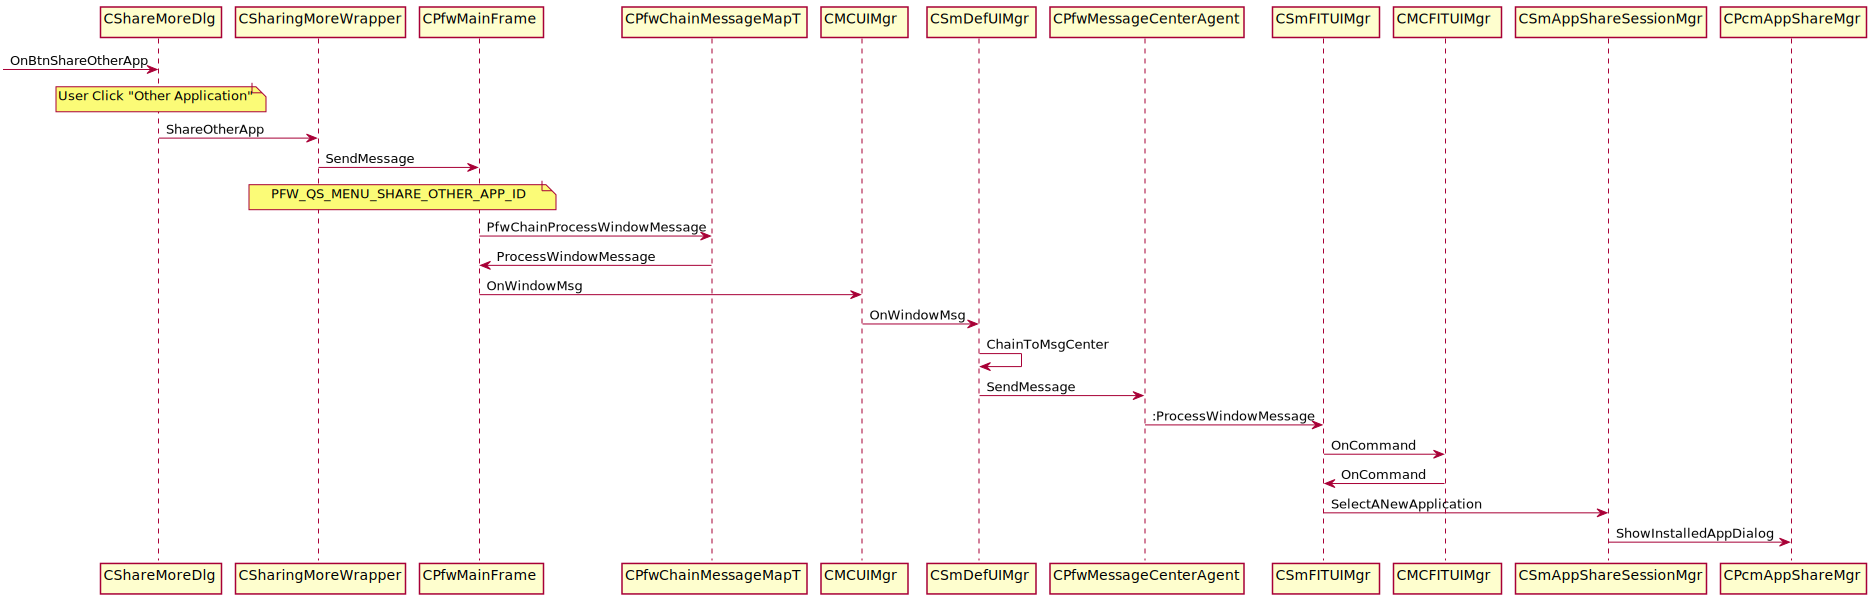
\includegraphics{quick_start_share_application_more_installed_dlg_seq.svg}


\section{Presenter Share Application}
\label{app_share:presenter-share-application}\begin{enumerate}
\item {} 
Share Application from \textbf{Application Share} dialog

\item {} 
Share Application from \textbf{Other Application} dialog

\item {} 
Share Application from menu \textbf{Share =\textgreater{} Application}

\item {} 
Share Application from quick start \textbf{More} menu

\end{enumerate}


\section{Attendee Notified Share Application}
\label{app_share:attendee-notified-share-application}

\chapter{Anyone can share}
\label{anyone_can_share:anyone-can-share}\label{anyone_can_share::doc}

\chapter{Record Privilege And Relevant UI}
\label{record_logic:record-privilege-and-relevant-ui}\label{record_logic::doc}
This document will show you:
\begin{itemize}
\item {} 
How the presenter \emph{`assign'} or \emph{`withdraw'} \textbf{record privilege}

\item {} 
How the attendee's UI behaviour will be changed when had assigned \textbf{record privilege}

\item {} 
How the attendee's UI behaviour will be changed when had withdrawer \textbf{record privilege}.

\end{itemize}


\section{Presenter \emph{`assign'} or \emph{`withdraw'} record privilege}
\label{record_logic:presenter-assign-or-withdraw-record-privilege}\begin{itemize}
\item {} 
Step1: Click \emph{`Menu=\textgreater{}Participant=\textgreater{}Assign Privilege ...'}

\item {} 
Step2: Show \emph{`Participant privilege'} dialog

\item {} 
Step3: In \emph{`Participant privilege'} dialog, Click \emph{`Participants'} tab

\item {} 
Step4: In \emph{`Participant'} tab, Check or UnCheck \emph{`Record a meeting'} check box

\item {} 
Step5: Then click \textbf{Assign} button

\end{itemize}

Here is the sequence:

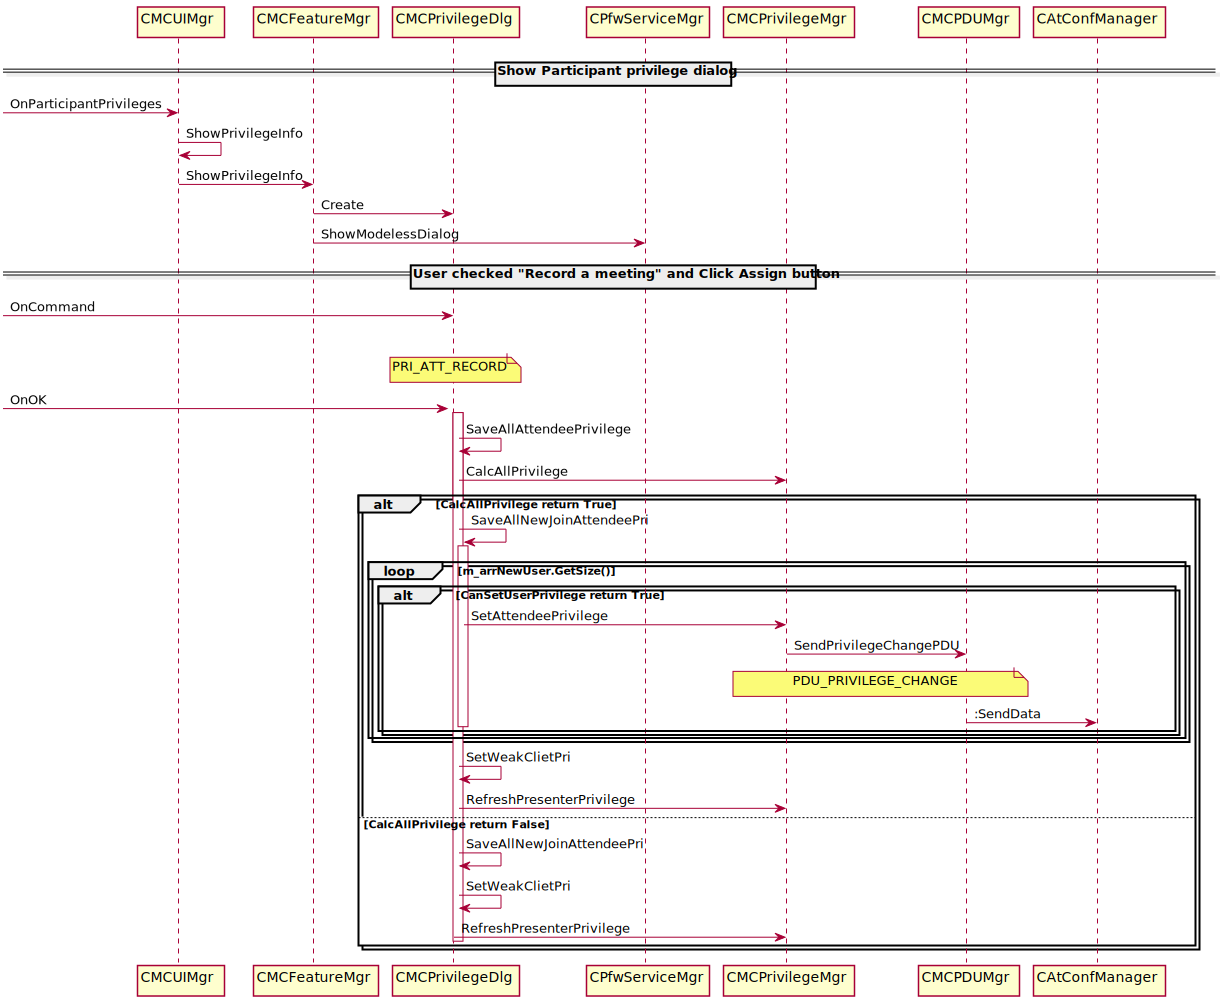
\includegraphics{record_presenter_assign_privilege_seq.svg}


\section{Show ``Save Recored Meeting As'' dialog}
\label{record_logic:show-save-recored-meeting-as-dialog}\begin{itemize}
\item {} 
Step1: Presenter assign the \emph{`Record Privilege'} to attendee

\item {} 
Step2: Attendee click \emph{`Record'} button from \emph{`Quick Start'}

\item {} 
Step3: Show \emph{`Save Recored Meeting As'} dialog

\end{itemize}

Here is the sequence show the call flow when the Attendee click \emph{`Record'} from \emph{`Quick Start'} :

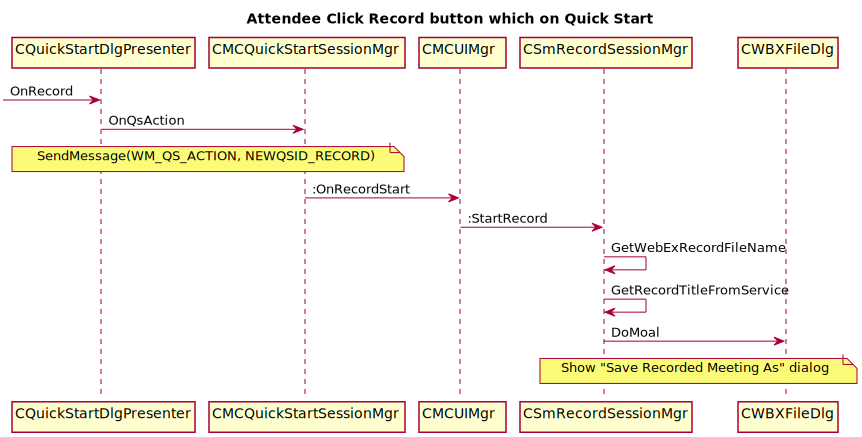
\includegraphics{record_attendee_click_seq.svg}


\section{Attendee receive a ``withdraw record privilege'' message}
\label{record_logic:attendee-receive-a-withdraw-record-privilege-message}
There are three case:
\begin{itemize}
\item {} 
Case1: Attendee without click \textbf{Record} from \emph{Quick Start}

\item {} 
Case2: Attendee clicked \textbf{Record} from \emph{Quick Start}, and showed \emph{`Save Recored Meeting As'} dialog

\item {} 
Case3: Attendee had \textbf{Recored} the meeting

\end{itemize}

When presenter withdraw the attendee's privilege, here is the sequence at the attendee side

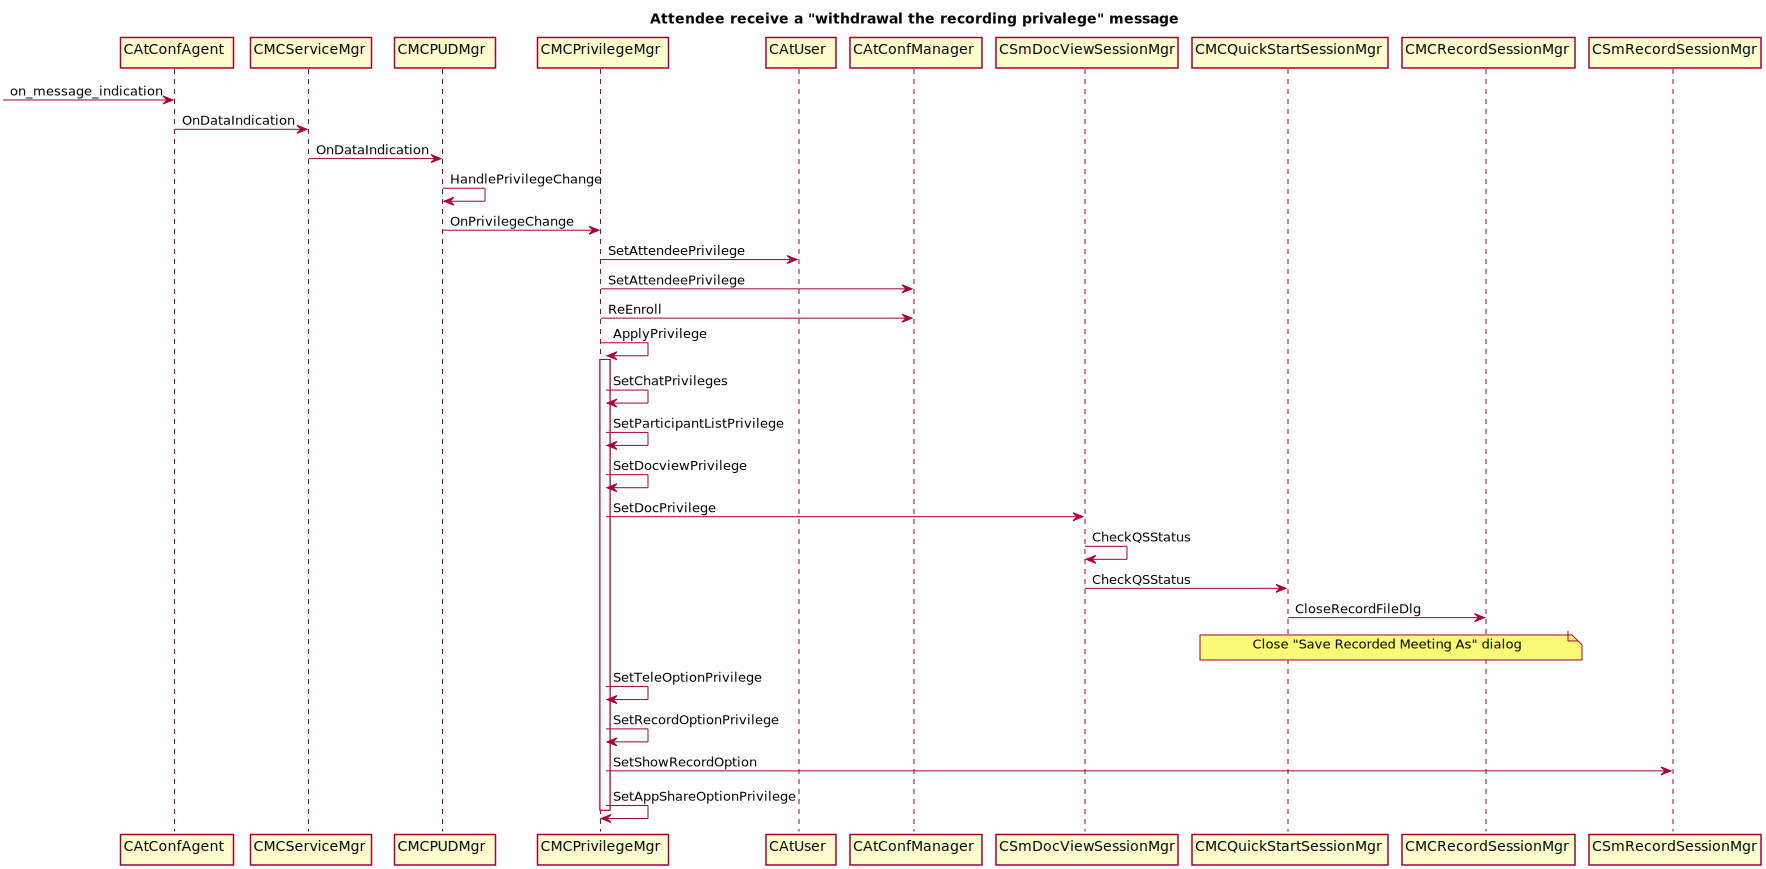
\includegraphics{record_attendee_withdrawal_privilege_seq.svg}


\chapter{PT Introduce}
\label{pt:pt-introduce}\label{pt::doc}

\section{Where is the PT}
\label{pt:where-is-the-pt}\begin{itemize}
\item {} 
Source code directory : 020p/src/windows/productivity\_tools

\item {} 
Project name : pt.sln

\item {} 
Installed Directory : c:\textbackslash{}Program Files (x86)\textbackslash{}WebEx\textbackslash{}Productivity Tools

\item {} 
MSI Package (office site) : You can download the package from \textbf{Meeting Center-\textgreater{}Downloads-\textgreater{}Productivity Tools}

\item {} 
MSI Package (dev or test site) : \href{http://ccatg-build2.cisco.com/cirepo/Train/T30L10N/client-T30L10N.383/delivery/WBXptool}{http://ccatg-build2.cisco.com/cirepo/Train/T30L10N/client-T30L10N.383/delivery/WBXptool}

\item {} 
PT download directory : c:\textbackslash{}Users\textbackslash{}xxx\textbackslash{}Roaming\textbackslash{}webex\textbackslash{}Productivity Tools

\end{itemize}


\section{PT Owner}
\label{pt:pt-owner}\begin{enumerate}
\item {} 
Allen Jia

\item {} 
Russell Chen

\end{enumerate}


\section{PT vs GPC}
\label{pt:pt-vs-gpc}\begin{itemize}
\item {} 
PT almost use MSI to install

\item {} 
PT use ptUpdate for upgrade

\item {} 
PT has its own code for version compare

\item {} 
PT's work directory defined after MSI installed

\end{itemize}

PT component diagram:

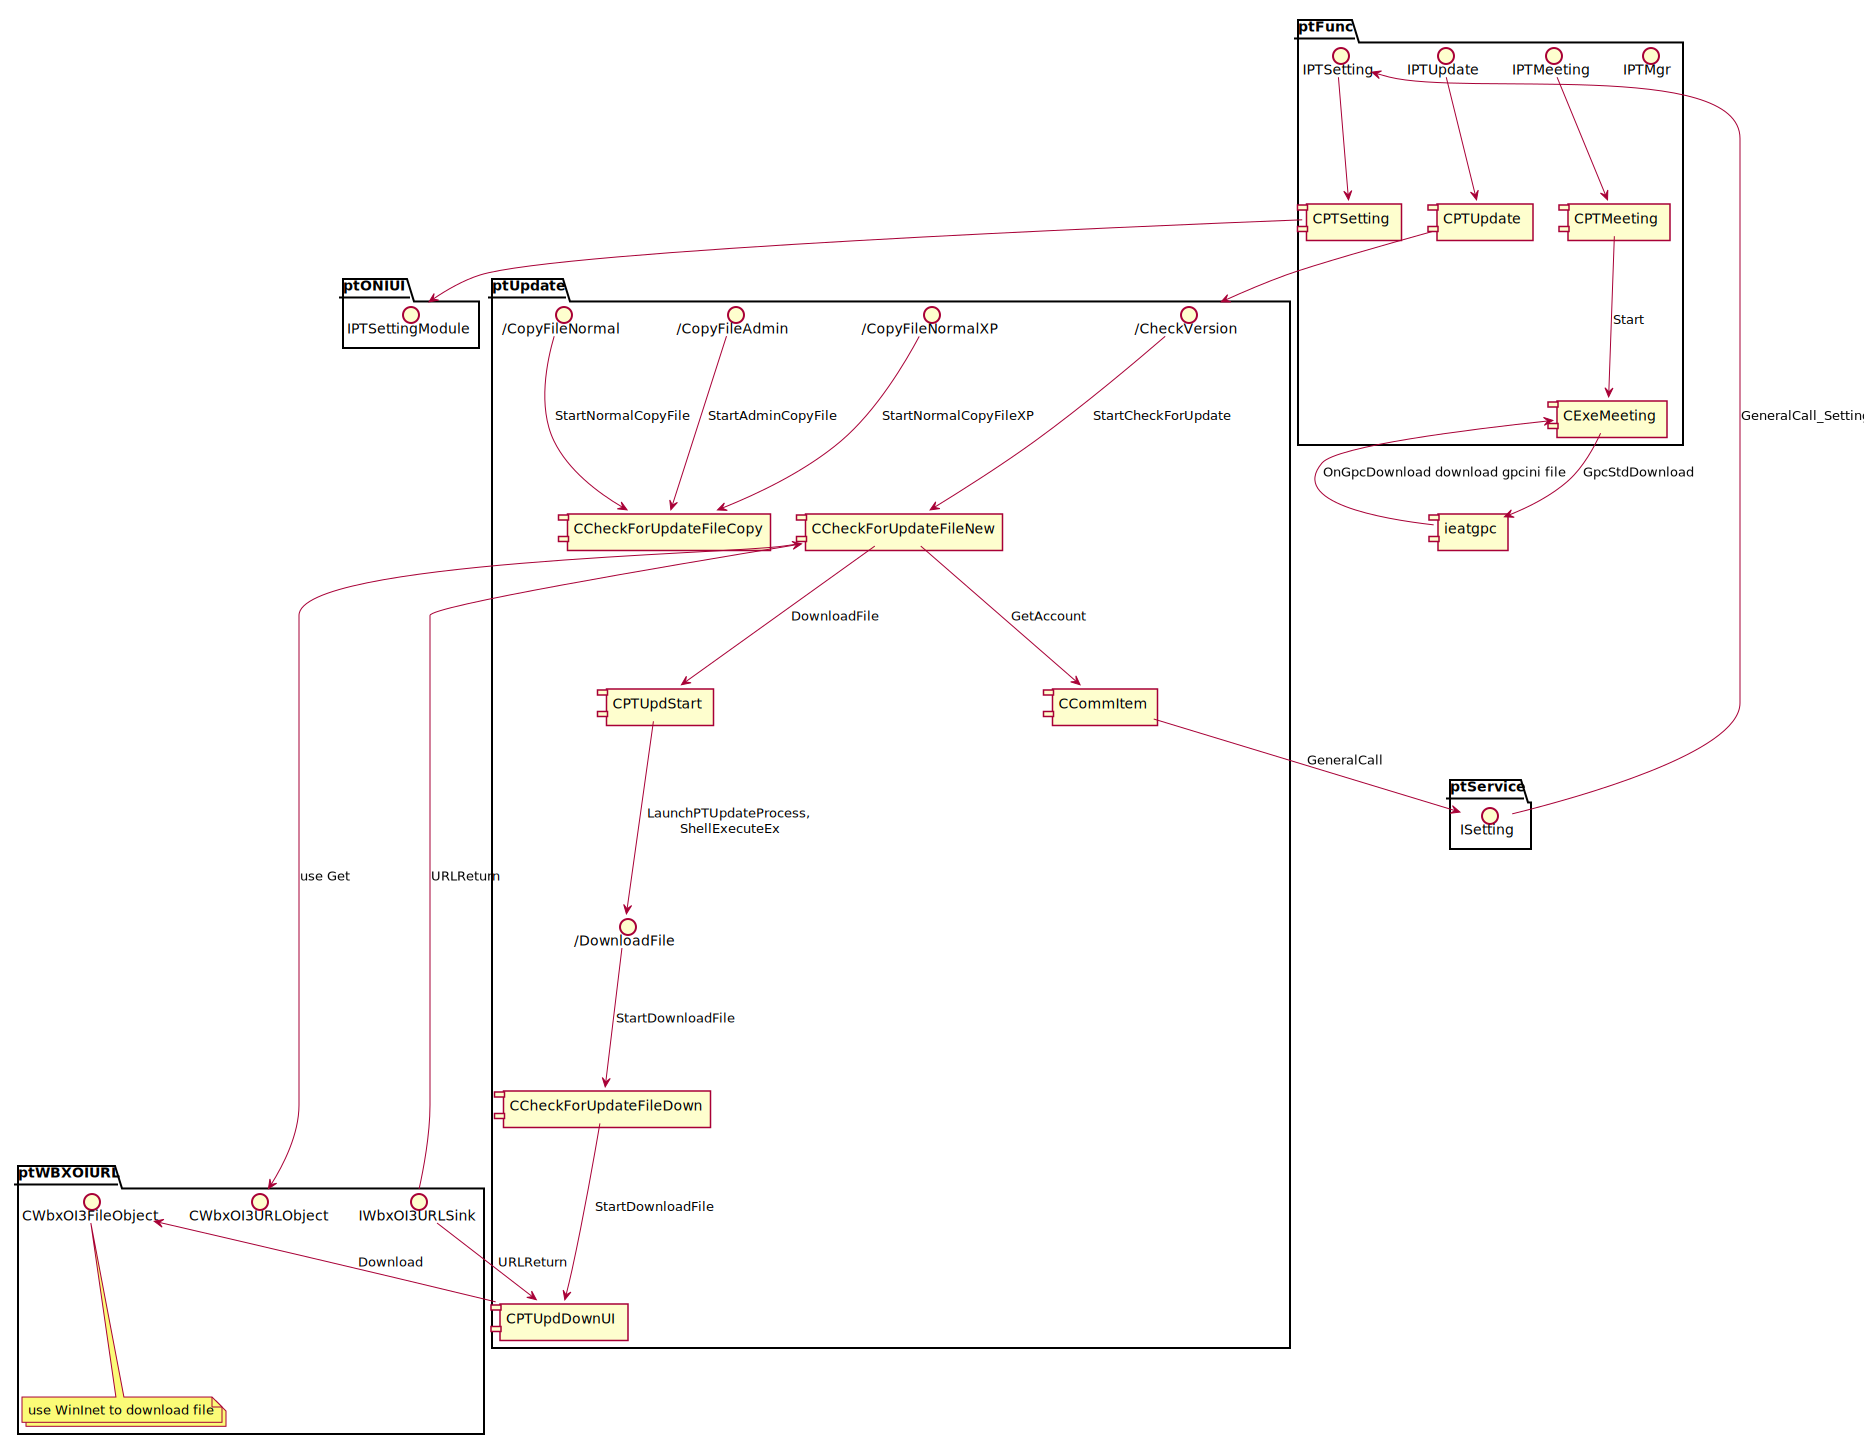
\includegraphics{pt_component.svg}


\subsection{ptUpdate Feature}
\label{pt:ptupdate-feature}\begin{itemize}
\item {} 
/CheckVersion

\item {} 
/DownloadFile

\item {} 
/CopyFileNormalXP

\item {} 
/CopyFileAdmin

\item {} 
/CopyFileNormal

\end{itemize}

Check version sequence diagram:

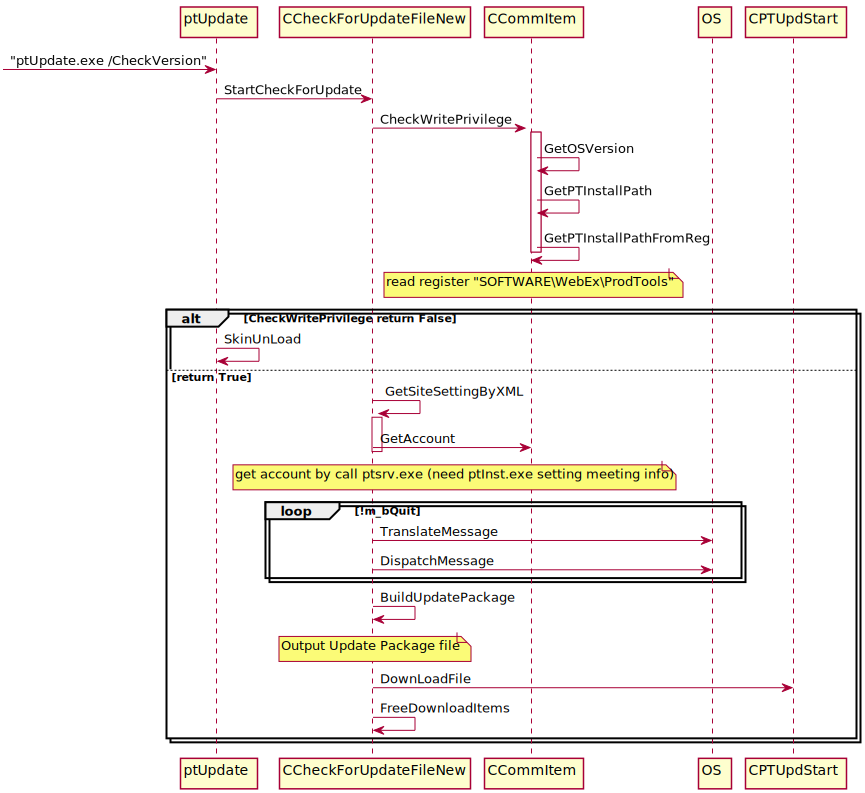
\includegraphics{ptupdate_check_version_seq.svg}

Check version status diagram:

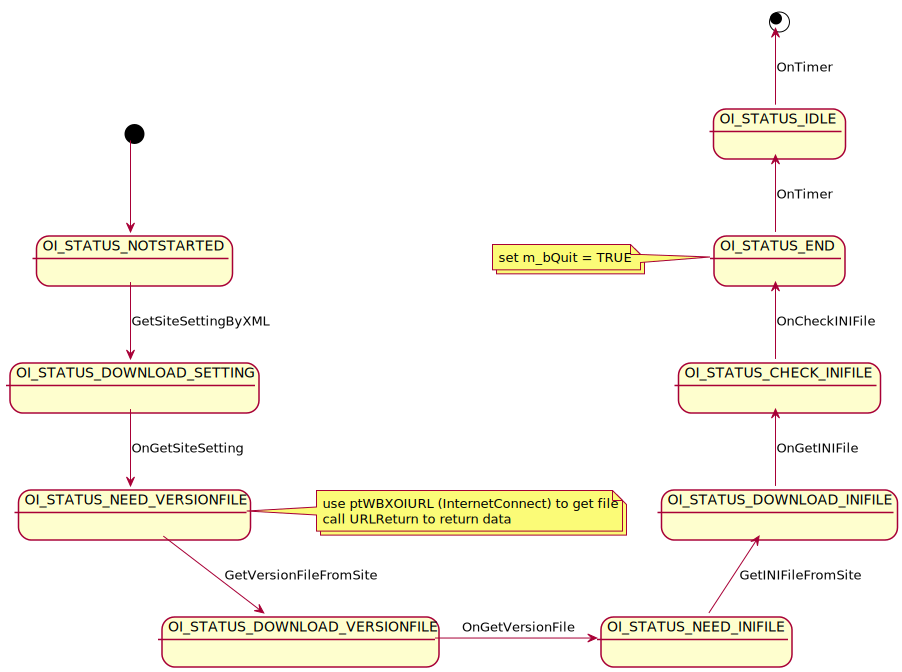
\includegraphics{ptupdate_oi_status_state.svg}


\section{PT Meeting With \textbf{Russell Chen}}
\label{pt:pt-meeting-with-russell-chen}\begin{enumerate}
\item {} 
Introduce PT basic knowledge

\end{enumerate}
\begin{quote}

\href{https://go.webex.com/go/lsr.php?RCID=bc459e215d0c47f8b4247550eb6ec79c}{https://go.webex.com/go/lsr.php?RCID=bc459e215d0c47f8b4247550eb6ec79c}
\end{quote}


\chapter{Indices and tables}
\label{index:indices-and-tables}\begin{itemize}
\item {} 
\emph{genindex}

\item {} 
\emph{modindex}

\item {} 
\emph{search}

\end{itemize}


\chapter{Title}
\label{index:title}


\renewcommand{\indexname}{Index}
\printindex
\end{document}
